\documentclass[a4paper,12pt]{article}
\usepackage[utf8]{inputenc}
\usepackage[T1]{fontenc}
\usepackage{lmodern}
\usepackage{geometry}
\usepackage{setspace}
\usepackage{fancyhdr}
\usepackage{hyperref}
\usepackage{amsmath}
\usepackage{amsfonts}
\usepackage{amssymb}
\usepackage{mathtools}
\usepackage{float}
\usepackage{tabularx}
\usepackage{enumitem}
\usepackage{graphicx}
\usepackage{ragged2e}
\usepackage[spanish]{babel}
\usepackage{booktabs}
\usepackage{longtable}
\usepackage{multirow}
\usepackage{xcolor}
\usepackage{microtype}
\usepackage{caption}
\usepackage{textcomp}
\newcommand{\euro}{\texteuro}
\newcommand{\E}{\mathbb{E}}
\newcommand{\Var}{\mathrm{Var}}
\newcommand{\Cov}{\mathrm{Cov}}
\newcommand{\VaR}{\mathrm{VaR}}
\newcommand{\TVaR}{\mathrm{TVaR}}
\addto\captionsspanish{\renewcommand{\tablename}{Tabla}}
\addto\captionsspanish{\renewcommand{\figurename}{Figura}}
\captionsetup{font=small,labelfont=bf}

% Configuración de márgenes
\geometry{left=2.5cm,right=2.5cm,top=3cm,bottom=3cm}

% Configuración de encabezados y pies de página
\pagestyle{fancy}
\fancyhf{}
\renewcommand{\headrulewidth}{0pt}
\fancyfoot[C]{\thepage}

% Configuración de interlineado
\onehalfspacing
\justifying

% Configuración de hipervínculos
\hypersetup{
    hidelinks,
    colorlinks=false
}

\begin{document}

% Primera página (Título, Resumen y Abstract)
\begin{titlepage}
    \centering
    \vspace*{0.1cm}
    \huge\textbf{Tema 1: Preguntas de debate}\\
    \vspace{1cm}
    \small{Luiz Alberto Luzuriaga Izquierdo}\\
    \vspace{0.1cm}
    Facultad de ciencias económicas, empresariales y turismo. \\
    \vspace{0.1cm}
    Universidad de Alcalá de Henares. \\
    \vspace{0.1cm}
    Curso 2026-2027\\
    \vspace{0.5cm}

{\bfseries Resumen}

\vspace{0.1cm}
\noindent
\begin{justify}
Respuestas argumentadas a las preguntas de debate del tema, con cifras de los casos prácticos. Tema 1 (Teoría de la utilidad y decisiones bajo riesgo): Funciones de utilidad CRRA y CARA, coeficiente de Arrow-Pratt, equivalente cierto, prima de riesgo y zona de acuerdo cedente-reasegurador.\\\\
\vspace{0.1cm}
\noindent
\textbf{Palabras clave}: utilidad esperada, aversión al riesgo, reaseguro, preguntas de debate.
\end{justify}
\begin{center}
    {\bfseries Abstract}
\end{center}
\vspace{0.1cm}
\noindent
\begin{justify}
Class work for Topic 1 of Actuarial Mathematics of Stability and Solvency of Insurance Activity: discussion questions with actuarial reasoning and numerical evidence.\\\\
\vspace{0.1cm}
\noindent
\textbf{Keywords}: expected utility, risk aversion, reinsurance, discussion questions.
\end{justify}

\end{titlepage}

% Índice
\newpage\pagenumbering{gobble}
\renewcommand{\contentsname}{Índice}
\newgeometry{left=4cm, right=4cm, top=3cm, bottom=2.5cm}
\tableofcontents

\restoregeometry
\newpage
\numberwithin{equation}{section}
\pagenumbering{arabic}
\setcounter{page}{1}

\section{Tema 1: Teoría de la utilidad y decisiones bajo riesgo}
\label{sec:tema1debate}
\noindent
Respuestas argumentadas a las preguntas de debate del tema, con cifras de los casos prácticos. Material de referencia: diapositivas del Tema 1 (Prof. Hugo González Riera).

\subsection{Debate 1 -- ?`Por qu\'e un reasegurador global puede ofrecer primas m\'as bajas que una aseguradora local?}

\paragraph{Tesis.} Porque su aversi\'on absoluta al riesgo $\alpha_R$ es menor que la de la aseguradora local, y la prima de riesgo es, en primera aproximaci\'on, proporcional a la aversi\'on. La menor aversi\'on es consecuencia econ\'omica de dos cosas que se confunden con frecuencia: \emph{capital} y \emph{diversificaci\'on}.

\paragraph{1. Lo que dice Arrow--Pratt.} Con $\pi\approx\tfrac12\,r\,\sigma^2$, para el mismo riesgo con $\sigma^2$ fijo la prima de riesgo escala con $r$. En el Caso~1, $\Var[X]=500.000$: con $\alpha_C=6\cdot10^{-4}$ el recargo aproximado es $\tfrac12\cdot6\cdot10^{-4}\cdot5\cdot10^5=150$ y con $\alpha_R=3\cdot10^{-4}$ es $75$. Las primas exactas (recargos de $18{,}9\%$ y $8{,}3\%$ sobre la pura de $1.000$) lo confirman: la aseguradora local no puede competir en precio con quien tiene la mitad de aversi\'on. La aproximaci\'on subestima el recargo exacto porque la Gamma es asim\'etrica y $\sigma^2$ no captura la cola.

\paragraph{2. Capital: la aversi\'on es tolerancia inversa.} La inversa $\tau=1/\alpha$ es la \emph{tolerancia al riesgo}, y se interpreta como la escala de p\'erdida que el decisor asume sin inmutarse (en el Caso~1, $\tau_C\approx1.667$ frente a $\tau_R\approx3.333$ miles de euros). Una entidad con el doble de fondos propios tiene, en esa lectura, la mitad de aversi\'on absoluta. Es la misma intuici\'on que justifica la CRRA: $r(w)=\gamma/w$ decrece con la riqueza.

\paragraph{3. Diversificaci\'on: un matiz que conviene no olvidar.} Con utilidad exponencial la prima de un riesgo independiente \emph{no} depende del resto de la cartera, porque $P(X+Y)=P(X)+P(Y)$. Es decir, que el reasegurador tenga muchos otros riesgos no abarata el precio de \emph{este} riesgo por s\'i solo; lo hace si hay \emph{dependencia} (cuando el riesgo ya forma parte de una cartera y su contribuci\'on marginal depende de $\mathrm{Cov}$) o si se interpreta que un reasegurador es un \emph{pool} de $m$ inversores: con $m$ aseguradores iguales con aversi\'on $\alpha$, la aversi\'on del grupo es $\alpha/m$ (suma de tolerancias, Borch, 1962). En ese sentido la diversificaci\'on \emph{mutualiza} el riesgo en un balance mucho mayor, y es esa mutualizaci\'on la que reduce $\alpha_R$.

\paragraph{4. Por qu\'e hay ganancias de intercambio.} Al ser $\alpha_R<\alpha_C$, existe una zona de acuerdo $[1.083{,}5;\,1.188{,}9]$ de anchura $105{,}5$: ceder el riesgo mejora la utilidad esperada de ambas partes. El reasegurador cobra por encima de lo que \emph{le} cuesta el riesgo y el cedente paga por debajo de lo que \emph{a \'el} le cuesta.

\paragraph{5. Matices que impiden concluir que el reasegurador siempre es m\'as barato.}
\begin{itemize}[leftmargin=*,itemsep=1pt]
\item \textbf{Costes que el modelo ignora}: gastos, margen de beneficio y coste del capital regulatorio (en Solvencia~II, margen de riesgo con tasa de coste del capital del $6\%$ sobre el SCR futuro). Estos costes se suman a $P^-$.
\item \textbf{Riesgo de contraparte y de base}: el cedente asume el riesgo de impago del reasegurador (que reduce el SCR de suscripci\'on pero introduce SCR de contraparte) y los riesgos de cobertura insuficiente.
\item \textbf{Correlaci\'on de colas}: un reasegurador global concentra eventos catastr\'ofico-clim\'aticos; tras un gran evento puede subir precios (mercado duro) y la ventaja de aversi\'on desaparece.
\item \textbf{Informaci\'on asim\'etrica}: la aseguradora local conoce mejor la calidad de su cartera; el reasegurador cobra una prima por selecci\'on adversa que no cabe en el modelo de utilidad.
\end{itemize}

\paragraph{Conclusi\'on.} El ahorro no procede de ``saber m\'as'' sino de tener una $\alpha_R$ menor gracias a capital y mutualizaci\'on; el ahorro es real mientras $\alpha_R<\alpha_C$ y se erosiona con costes, correlaci\'on de colas y riesgo de contraparte.

\bigskip\hrule\bigskip

\subsection{Debate 2 -- Un apetito de riesgo declarado incoherente con la aversi\'on impl\'icita}

\paragraph{Tesis.} Si lo que la entidad declara en el ORSA no es compatible con lo que realmente hace al reasegurar e invertir, el apetito de riesgo es un papel y no un instrumento de gobierno. Esto genera riesgos de tres tipos: de gobernanza, de capital y de supervisi\'on.

\paragraph{C\'omo se mide la aversi\'on impl\'icita.} La aversi\'on impl\'icita $\alpha_{\text{impl}}$ es la que reproduce el precio realmente aceptado. En el Caso~1, si la cedente declara en el ORSA una aversi\'on correspondiente al reasegurador ($\alpha=3\cdot10^{-4}$, que justifica pagar hasta $P=1.083{,}5$) pero en la pr\'actica paga $1.150$ por ceder el 100\,\%, se resuelve $\ln M_X(\alpha)/\alpha=1.150$ y se obtiene $\alpha_{\text{impl}}\approx5\cdot10^{-4}$, un $66\%$ superior a la declarada. Con $P=1.188{,}9$ se alcanzar\'ia $6\cdot10^{-4}$, el valor del cedente. La brecha $\alpha_{\text{impl}}/\alpha_{\text{decl}}$ es un indicador cuantitativo f\'acil de monitorizar.

\paragraph{Riesgos de gobernanza.}
\begin{itemize}[leftmargin=*,itemsep=1pt]
\item \textbf{El apetito deja de gobernar.} Los l\'imites (retenci\'on por l\'inea, l\'imites de inversi\'on) se fijan pensando en una aversi\'on y se ejecutan con otra; la alta direcci\'on cree que toma menos riesgo del que toma realmente. El ORSA pierde su funci\'on de enlazar estrategia, riesgo y capital.
\item \textbf{Incentivos (agencia).} Los directivos con retribuci\'on convexa (bonus sin penalizaci\'on por p\'erdidas) tienen una utilidad efectiva menos c\'oncava que la de los accionistas o asegurados: act\'uan con $\alpha_{\text{impl}}<\alpha_{\text{decl}}$. Si el apetito declarado es muy conservador y la retribuci\'on empuja a lo contrario, el sesgo ser\'a sistem\'atico.
\item \textbf{Sobrerreaseguro costoso.} El caso inverso ($\alpha_{\text{impl}}>\alpha_{\text{decl}}$) significa pagar por ceder m\'as de lo que la estrategia justifica: erosiona el margen y se mantiene porque ``cubrirse nunca es criticable''.
\end{itemize}

\paragraph{Riesgos de capital.} Con aversi\'on subestimada se asume m\'as riesgo del dotado por el SCR calculado con el perfil declarado: el capital econ\'omico propio puede quedarse por debajo del necesario para la ambici\'on real. Con aversi\'on sobreestimada se inmoviliza capital que podr\'ia remunerarse.

\paragraph{Riesgos de supervisi\'on (Solvencia~II).} La directiva exige un sistema de gobernanza eficaz, y el ORSA debe ser una herramienta de gesti\'on usada en las decisiones estrat\'egicas (``use test'' en modelo interno). Si el supervisor detecta incoherencia entre el apetito, la pol\'itica de reaseguro y el perfil de riesgo real, puede cuestionar la validez del ORSA, exigir medidas correctoras sobre la gobernanza y, en casos graves, imponer un recargo de capital por deficiencias de gobierno del sistema de gesti\'on. Tambi\'en afecta a la credibilidad de un modelo interno: un modelo cuya salida no se usa en las decisiones puede perder la autorizaci\'on.

\paragraph{Qu\'e har\'ia en la pr\'actica.} (i) Calibrar y documentar $\alpha$ o $\gamma$ de la entidad (a partir de fondos propios, tolerancia a la ca\'ida del ratio de solvencia o apetito en t\'erminos de VaR); (ii) contrastarlo \emph{ex post} con las decisiones realmente tomadas mediante el indicador $\alpha_{\text{impl}}/\alpha_{\text{decl}}$; (iii) elevar al Consejo cualquier desviaci\'on sostenida; (iv) alinear la retribuci\'on con el apetito.

\bigskip\hrule\bigskip

\subsection{Debate 3 -- Caso 2 con $\gamma=1$ (utilidad logar\'itmica)}

\paragraph{C\'alculo.} Con $w=10.000$ y $X=+2.000$ o $-1.500$ con probabilidad $1/2$, la riqueza final es $12.000$ u $8.500$. Para $\gamma=1$, el CE es la media geom\'etrica:
\[
CE=\exp\!\big(\tfrac12\ln12.000+\tfrac12\ln8.500\big)=\sqrt{12.000\cdot8.500}=10.099{,}5.
\]
Como $CE>w=10.000$, la prima de riesgo es $\pi=10.250-10.099{,}5=150{,}5<250$: \textbf{el gestor acepta} la posici\'on. Con $\gamma=3$ (enunciado) el CE era $9.809{,}3$ y rechazaba; la decisi\'on se invierte al rebajar la aversi\'on.

\paragraph{Umbral.} El valor cr\'itico $\gamma^*$ que anula el beneficio del gestor es la ra\'iz de $CE(\gamma)=w$: $\gamma^*\approx1{,}668$. Aceptan, por tanto, los perfiles con $\gamma<1{,}67$ (incluyendo el logar\'itmico y el agresivo con $\gamma=0{,}5$, $CE=10.174{,}8$) y rechazan los de $\gamma\ge2$ ($CE=9.951{,}2$ para $\gamma=2$).
\begin{figure}[H]\centering
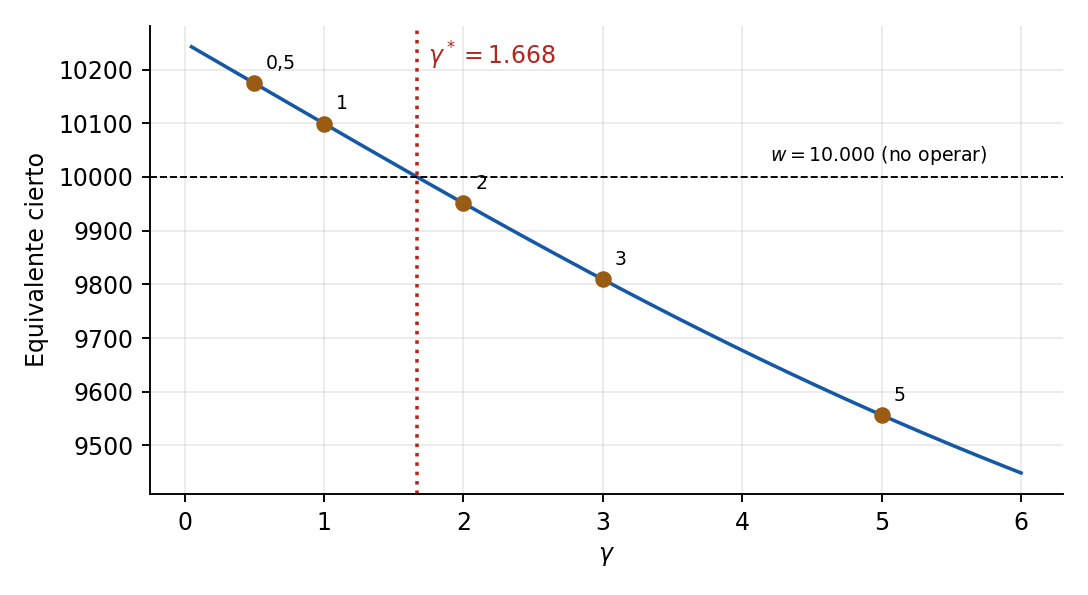
\includegraphics[width=.74\linewidth]{t1_f_debate3.png}
\caption{Equivalente cierto del Caso~2 frente a $\gamma$; la decisi\'on cambia en $\gamma^*\approx1{,}668$.}
\end{figure}

\paragraph{?`Qu\'e perfil tiene $\gamma\approx1$?} El valor $\gamma=1$ es el extremo agresivo de la banda emp\'irica $[1,10]$. Cabe esperarlo en:
\begin{itemize}[leftmargin=*,itemsep=1pt]
\item \textbf{Inversores de horizonte largo, muy capitalizados y sin restricciones de liquidez}: fondos soberanos, grandes fondos de pensiones de capitalizaci\'on, \emph{endowments}. Maximizar la utilidad logar\'itmica es el criterio de crecimiento \'optimo (Kelly) y para ellos las p\'erdidas son transitorias.
\item \textbf{Familias o entidades con balance mucho mayor que la posici\'on}: si el riesgo es peque\~no respecto de la riqueza total, la aversi\'on efectiva es baja. Aqu\'i la clave es que $w=10.000$ es el capital \emph{asignado a la mesa}, no el del banco: si se midiera sobre todo el balance el riesgo ser\'ia irrelevante y cualquier $\gamma$ moderado aceptar\'ia.
\item \textbf{Mesas propietarias con tolerancia expl\'icita al riesgo}, con l\'imites de p\'erdida pero retribuci\'on ligada al resultado.
\end{itemize}
No cabe esperarlo en bancos reguladores con requisitos de capital, en entidades de dep\'ositos o en aseguradoras de vida con garant\'ias: ah\'i la regulaci\'on (SCR, MCR, colchones) y la reputaci\'on obligan a trabajar con $\gamma$ efectivamente alto.

\paragraph{Un matiz.} Seg\'un la regla de Merton, la fracci\'on \'optima en el activo con riesgo es $\mu/(\gamma\sigma^2)$: pasar de $\gamma=3$ a $\gamma=1$ \emph{triplica} la exposici\'on deseada. Ese cambio de $\gamma$ no es un detalle: es multiplicar por tres el apetito de riesgo; un comit\'e de riesgos debe verlo as\'i.

\bigskip\hrule\bigskip

\subsection{Debate 4 -- ?`Importa solo la riqueza final?}

\paragraph{Tesis.} La utilidad esperada sobre la riqueza final asume que no importa el trayecto ni cu\'ando se cobra o paga. En gesti\'on de solvencia esto falla cuando hay \textbf{barreras}, \textbf{iliquidez} o \textbf{horizonte distinto del de decisi\'on}.

\paragraph{Situaciones donde es m\'as cuestionable.}
\begin{enumerate}[leftmargin=*,itemsep=2pt]
\item \textbf{Liquidez y ventas forzadas.} Dos carteras con la misma riqueza final pueden tener trayectorias muy distintas: la que sufre una ca\'ida intermedia puede enfrentarse a \emph{margin calls} o a rescates y vender activos a precios de saldo. Casos: marzo de 2020, o la crisis de los fondos LDI en el Reino Unido (septiembre de 2022), donde fondos de pensiones solventes a vencimiento tuvieron problemas de liquidez en el camino. Para la utilidad esperada ambas trayectorias son id\'enticas.
\item \textbf{Barreras regulatorias.} Si el ratio de solvencia cae por debajo del $100\%$ del SCR o del MCR, el supervisor interviene y se pierde el control de la entidad. La utilidad de la entidad ``salta'' (se hunde) al cruzar el umbral: $u$ ya no es c\'oncava y suave sino que tiene una barrera en $w=L$. En el Caso~2, por ejemplo, un l\'imite de p\'erdida de la mesa en $9.000$ rechazar\'ia la posici\'on para \emph{cualquier} $\gamma$, porque el escenario desfavorable ($8.500$) la cruza.
\item \textbf{Horizonte.} Solvencia~II mide a un a\~no al $99{,}5\%$ ($VaR$), mientras que un producto de vida a 30 a\~nos o un fondo de pensiones tiene obligaciones a muy largo plazo. Con ajustes como el de casamiento o el de volatilidad, el mismo balance puede ser ``insolvente'' en el a\~no y solvente al vencimiento: la riqueza final no es lo que se vigila.
\item \textbf{Referencia y p\'erdidas (teor\'ia prospectiva).} Gerentes y accionistas valoran los resultados respecto a un punto de referencia (presupuesto, ejercicio anterior, rating) y son m\'as sensibles a las p\'erdidas que a las ganancias (Kahneman y Tversky, 1979). Un banco que arrastra p\'erdidas puede asumir m\'as riesgo para ``recuperar'': comportamiento opuesto al averso.
\item \textbf{Contabilidad y resultados intermedios.} En IFRS~17 el margen de servicio contractual se libera en el tiempo y los flujos intermedios pesan en los resultados publicados; la utilidad del gestor depende de la senda del beneficio, no solo del valor econ\'omico final.
\item \textbf{Cl\'ausulas de ca\'ida (\emph{cross-default}, ratings).} Una rebaja de calificaci\'on por debajo de un umbral cambia los costes de financiaci\'on y las garant\'ias exigidas: otro salto no capturado.
\end{enumerate}

\paragraph{C\'omo se corrige en la pr\'actica.} (a) Con una funci\'on de utilidad con barrera o penalizaci\'on cuando $w<L$, o convirtiendo el problema en uno con restricci\'on de probabilidad de ruina ($\Pr[W<L]\le\varepsilon$), lo que es en la pr\'actica lo que hace el VaR de Solvencia~II. (b) Con modelos multiper\'iodo (programaci\'on din\'amica, utilidad recursiva de Epstein--Zin, que separa aversi\'on al riesgo y preferencia temporal). (c) Con \emph{stress tests} de liquidez y escenarios de trayectoria, que son justamente los que la utilidad sobre riqueza final no ve.

\paragraph{Conclusi\'on.} El modelo VNM sigue siendo \'util como primera aproximaci\'on para decisiones puntuales y de riesgo ``moderado'', pero la gesti\'on de solvencia es un problema de \emph{trayectoria con restricciones}: liquidez, barreras y horizonte. La pista del enunciado (liquidez y horizonte temporal) apunta exactamente a ello.

\subsubsection*{Referencias}
\begin{itemize}[leftmargin=*,itemsep=0pt]
\item Kaas, R., Goovaerts, M., Dhaene, J. y Denuit, M. (2008). \emph{Modern Actuarial Risk Theory} (2.\textordfeminine\ ed.). Springer.
\item Borch, K. (1962). Equilibrium in a reinsurance market. \emph{Econometrica}, 30, 424--444.
\item Kahneman, D. y Tversky, A. (1979). Prospect theory. \emph{Econometrica}, 47, 263--291.
\item Merton, R. C. (1969). Lifetime portfolio selection under uncertainty. \emph{Review of Economics and Statistics}, 51, 247--257.
\item Directiva 2009/138/CE (Solvencia~II); NIIF~17 Contratos de seguro.
\end{itemize}

\end{document}
